%%%%%%%%%%%%%%%%%%%%%%%%%%%%%%%%%%%%%%%%%
% Short Sectioned Assignment
% LaTeX Template
% Version 1.0 (5/5/12)
%
% This template has been downloaded from:
% http://www.LaTeXTemplates.com
%
% Original author:
% Frits Wenneker (http://www.howtotex.com)
% Edited by Alice Wu
%
% License:
% CC BY-NC-SA 3.0 (http://creativecommons.org/licenses/by-nc-sa/3.0/)
%
%%%%%%%%%%%%%%%%%%%%%%%%%%%%%%%%%%%%%%%%%

%----------------------------------------------------------------------------------------
%	PACKAGES AND OTHER DOCUMENT CONFIGURATIONS
%----------------------------------------------------------------------------------------

\documentclass[paper=letter, fontsize=11pt, twocolumn]{scrartcl} % letter and 11pt font size
\usepackage[margin=1in]{geometry}
\usepackage[T1]{fontenc} % Use 8-bit encoding that has 256 glyphs
\usepackage{fourier} % Use the Adobe Utopia font for the document - comment this line to return to the LaTeX default
\usepackage[english]{babel} % English language/hyphenation
\usepackage{amsmath,amsfonts,amsthm} % Math packages
\usepackage{comment}
\usepackage{graphicx}
\usepackage{caption}
\usepackage{subcaption}

\usepackage{lipsum} % Used for inserting dummy 'Lorem ipsum' text into the template
\usepackage{multirow}
\usepackage{sectsty} % Allows customizing section commands
\usepackage{fancyhdr} % Custom headers and footers
\pagestyle{fancyplain} % Makes all pages in the document conform to the custom headers and footers
\fancyhead{} % No page header - if you want one, create it in the same way as the footers below
\fancyfoot[L]{} % Empty left footer
\fancyfoot[C]{} % Empty center footer
\fancyfoot[R]{\thepage} % Page numbering for right footer
\renewcommand{\headrulewidth}{0pt} % Remove header underlines
\renewcommand{\footrulewidth}{0pt} % Remove footer underlines
%\setlength{\headheight}{0pt} % Customize the height of the header

\numberwithin{equation}{section} % Number equations within sections (i.e. 1.1, 1.2, 2.1, 2.2 instead of 1, 2, 3, 4)
%\numberwithin{figure}{section} % Number figures within sections (i.e. 1.1, 1.2, 2.1, 2.2 instead of 1, 2, 3, 4)
%\numberwithin{table}{section} % Number tables within sections (i.e. 1.1, 1.2, 2.1, 2.2 instead of 1, 2, 3, 4)

\setlength\parindent{20pt} % Removes all indentation from paragraphs - comment this line for an assignment with lots of text

%use itlesec package and zero out all the spaces and set it manually
%titlespacing are command, left margin, above-skip and below-kip respectively
\usepackage[compact]{titlesec}
\titlespacing{\section}{0pt}{*2}{*1}
\titlespacing{\subsection}{0pt}{*2}{*1}
\titlespacing{\subsubsection}{0pt}{*2}{*1}

%----------------------------------------------------------------------------------------
%	TITLE SECTION
%----------------------------------------------------------------------------------------

\newcommand{\horrule}[1]{\rule{\linewidth}{#1}} % Create horizontal rule command with 1 argument of height

\title{	
\normalfont \normalsize 
\textsc{Stanford University, CS229 - Machine Learning} \\ [10pt] % Your university, school and/or department name(s)
\horrule{0.5pt} \\[10pt] % Thin top horizontal rule
\begin{center}
\LARGE Don't Get Kicked - Machine Learning Predictions for Car Buying \\ % The assignment title
\end{center}
\horrule{2pt} \\[10pt] % Thick bottom horizontal rule
}

\author{Albert Ho, Robert Romano, X. Alice Wu} % Your name

\date{\normalsize\today} % Today's date or a custom date

\begin{document}
\noindent
\maketitle % Print the title

%----------------------------------------------------------------------------------------
%	PROBLEM 1
%----------------------------------------------------------------------------------------
\section{Introduction}
	When you go to an auto dealership with the intent to buy a used car, you want a good selection to choose from and you want to be able to trust the condition of the car that you buy. Auto dealerships purchase many of their used cars through auto auctions with the same goals that you have: they want to buy as many cars as they can in the best condition possible. The problem that these dealerships often face is the risk of buying used cars that have serious issues, preventing them from being sold to customers. These bad purchases are called "kicks", and they can be hard to spot for a variety of reasons. Many kicked cars are purchased due to tampered odometers or mechanical issues that could not be predicted ahead of time. For these reasons, car dealerships can benefit greatly from the predictive powers of machine learning. If there is a way to determine if a car would be kicked a priori, car dealerships can not only save themselves money, but also provide their customers with the best inventory selection possible.
	The following paper is split up into 5 main sections describing our approach to solve this problem: Initial Data Preprocessing, Early Algorithm Selection, Data Normalization and Balancing, Performance Evaluation, and Boosting. First we identified the key characteristics of our data and formed strategies for preprocessing. Next, we ran several simple machine learning algorithms. This led us to update our data processing strategy and determine a better way to evaluate and compare different learning algorithms. Finally, we implemented boosting and tailored our final algorithm selection based on initial successes.

\section{Initial Data Preprocessing}
	We obtained our data set from the Kaggle.com challenge "Don't Get Kicked" hosted by Carvana. The data set contained 32 unique features with 73,041 samples along with a labeling of 0 for good car purchases and 1 for "kicks". Some key features included odometer readings, selling prices, vehicle age, and vehicle model. One thing that we immediately noticed was that good cars were heavily overrepresented in the data set, representing 87.7\% of samples. The consequences of this became more apparent once we began comparing machine learning algorithms across different metrics. 

\subsection{Word Bins}
	Our first major challenge was the preprocessing of data. For data such as the name of the vehicle's model, manufacturer, and color, we had to assign unique identifiers to specific strings in the feature space. This was straightforward for a feature like transmission since we could assign 0 for Auto and 1 for Manual. The process became more involved with multivariate features such as the car submodel. We decided that even though there were many different submodels, categorizing them with unique identifiers rather than grouping them was the more conservative option.

\subsection{Missing Features}
	Some of the samples had missing features. We had the option of throwing out the sample completely, but we believed that it would be a waste. We decided to implement the following rules: if the feature was represented with a continuous value, we would replace the missing value with the average of the feature over the other samples and if the feature was represented with a discrete value, we would create a new value specifically to identify missing data.

\subsection{Data Visualization}
	Before running any algorithms, we visualized the data with plots to gain some intuition about the features. The training data was separated into good and bad datasets and compared, looking for trends. Histograms were plotted over each feature with the frequency normalized so that good and bad cars were equally represented. This allowed comparison of the relative frequency over a feature. An example is Figure 1a, showing that bad cars were generally older. To get an idea of how discriminating a feature was, the ratio of the relative frequency of bad to good was plotted. An example of this is Figure 1b, which showed that the older a car was the stronger the feature. Similarly, Figure 1c shows that Current Auction Average Price was a strong feature, however this needed to be taken with a grain of salt because the areas where the features were most discriminating were generally in small tail regions that applied to a very small subset of cars.

\section{Early Algorithm Selection}
	With the data parsed and some initial insights to guide us, we applied some basic machine learning algorithms that would identify where we needed improvement and what strategy would be most effective. At this point, we chose generalization error as a metric to evaluate our algorithms� performances.

\subsection{Support Vector Machine}
	First, we tested our data with an SVM. We used libLINEAR v. 1.92 and the method of cross validation by training on 70\% of our data set and testing on the remaining 30\%. Initial runs yielded about 12\% generalization error, which on first glance was very good. 

\subsection{Logistic Regression}
	Since the feature we were trying to predict was binary, we decided to try a logistic regression model as a first pass. Logistic regression via Newton's method was implemented in MATLAB with the same method of cross validation as that in SVM. We found that the algorithm converged after 7 iterations, yielding a generalization error of about 12\%.

\subsection{Observations}
	Using generalization error as a metric, both logistic regression and SVM seemed to have yielded promising results. Upon further investigation, however, these runs would nearly always predict the null hypothesis, i.e. a good car prediction for every testing sample. This was where we started to question the use of generalization error as a performance metric in favor of performance metrics that took into account false positives and false negatives. We also conducted a literature review in hopes of finding alternative algorithms more suitable for skewed data sets.

\section{Data Normalization and Balancing}
\subsection{Feature Normalization}
	After evaluating the performance of our early attempts, we made several changes to the data preprocessing procedure in hopes of achieving better results. Through our literature search, we found that data normalization increases the performance of many classification algorithms \cite{Graf} As a result, we normalized our numeric features over the range 0 to 1.

\subsection{Data Balancing}
	In addition to data normalization, we also discovered that "up-sampling" the data from the minority class is an effective way of solving the class imbalance problem. (\cite{Menardi}, \cite{Provost}, \cite{Japkowicz}). To do this we again split our data in a 70/30 cross-validation scheme. From the data split intended for training, we created a balanced training data set by oversampling the bad cars. Both balanced and unbalanced data sets were used for the algorithms we tested from this point forward to observe the effects of artificial data balancing.

\section{Performance Evaluation}
	As mentioned earlier, we found that using generalization error alone as a performance metric was misleading due to the bias of our data towards good cars. A prediction of all good cars, for example, would yield 12.3\% accuracy. In the context of our problem, it is more relevant to evaluate an algorithm�s performance based on (defined as TP/TP+FP) and recall(defined as TP/TP+FN) than predictive accuracy, since the number of false positive (FP) and false negatives (FN) predicted by an algorithm is more directly related to monetary loss and opportunity cost, which is ultimately what car dealers care about. In a case where all predictions are for good cars, precision is undefined (0/0) because there are no bad car predictions whereas Recall turns out to be 0 for the same reason. In general, you want a good balance between Precision and Recall. An increase in both indicates better performance between algorithms.
	Through our literature search, we found that when studying problems with imbalanced data, using the classifiers produced by standard machine learning algorithms without adjusting the output threshold may cause poor performance \cite{Provost}. In this respect, AUC is a good metric since it takes into account sensitivity (recall) and specificity over the entire range of possible output threshold values. AUC is then a good indicator of one classifier's ability for correct prediction over another. In addition, we also used the F1 score as a performance metric to account for the inverse relationship between precision and recall. (http://www.hpl.hp.com/techreports/2009/HPL-2009-359.pdf) We define F1 as the harmonic mean between precision and recall (2*precision*recall/(precision+recall)). If precision and recall has been traded off, the F1 score will not change. That way we can identify a superior algorithm as one that increases both precision and recall.

\section{Boosting}
	After applying data normalization and balancing, we returned to our initial approaches using SVM and logistic regression. We found that by using these algorithms with normalized and balanced data sets, we were able to achieve better AUC and F1 scores, and therefore better results than before. We also tried tuning the C parameter in libLINEAR to little effect. From our own research and discussion with the TAs, we found that boosting might be a promising approach for our learning problem. The idea behind boosting is to combine many weak learners into a strong learner (CITATION NEEDED). To implement boosting, along with a slew of other learning algorithms, we used Weka (Waikato Environment for Knowledge Analysis) v. 3.7.7.
	Weka made it easy to try many different learning algorithms quickly. Due to the nature of our data, we were very interested in comparing the performance of traditional classification algorithms with meta-classifiers such as boosting and ensemble learning. However, Weka is also very memory intensive. The program could not run logistic regression without crashing even with 5.0GB of memory allocated. As a result, logistic regression was still implemented in MATLAB, while all others were implemented in Weka.

\section{Results}
	We used Weka to implement several meta-classifiers, specifically AdaBoostM1, RealAdaBoost, LogitBoost, and ensemble selection. The weak classifiers we used were decision stump, decision table, REPTree, J48, and naive bayes. Decision stump is a one level decision tree. Decision table is a simple majority classifier. REPTree is a fast decision tree learner, based on information gain and pruning using reduced-error pruning with backfitting.  J48 is an implementation of the C4.5 decision tree, which is based on maximizing information gain.
	AdaBoostM1 is a general nominal classifier boosting algorithm. Using decision stump as its classifier, it performed reasonably well with an AUC of 0.724. We tried using more sophisticated classifiers such as J48, random forest, and REPTree, however they all performed worse. RealAdaBoost is an implementation of AdaBoost that is optimized for binary classification. Using decision stump as its classifier, it performed well with an AUC of 0.744. Similarly, other more sophisticated classifiers did worse, perhaps due to overfitting. LogitBoost using decision stump performed better than AdaBoostM1, with an AUC of 0.746. LogitBoost using decision table performed slightly better, with an AUC of .758. Because of this we decided to stick with logitBoost as our boosting algorithm of choice.
	Ensemble selection can use any combination of weak classifiers to make a strong classifier, so it is very flexible. One implementation is to additively build a strong classifier by selecting the strongest weak classifier, and then one by one adding the next strongest weak classifier. We chose to use AUC as the metric for evaluating classifier strength. Because ensemble selection uses a greedy optimization algorithm, it is prone to overfitting. To overcome this, strategies such as model bagging, replacement, and sort initialization were used. Ten model bags were used as well as sort initialization.
	The ensemble selection algorithm with most promise was one that incorporated many different classifiers, including naive bayes, J48, and REPTree classifiers. This resulted in an AUC of .749 when tested on the balanced data set along with an F1 of 0.279, just shy of LogitBoost.
	It was found that contrary to literature, balancing the data did not generally improve classifier performance. In fact, classifiers generally performed considerably worse.

\section{Discussion}
	We found through our investigation that LogitBoost was the best at predicting whether or not  a car would be a kick. It produced a prediction with the highest AUC value of 0.758 and an F1 of 0.368. The F1 value was not as high as we would have liked, but depending on the relationship between GrossProfit and Loss in the TotalProfit equation, F1 may not even be a great metric to maximize the parameter of interest.
	%TotalProfit = TN*Gross_Profit + FN*Loss
	%OpportunityCost = FP*Gross_Profit
	TotalProfit represents the profit that a car dealership will make if they follow the predictions of an algorithm. All cars that are classified as good and are actually good will make the dealership some average profit per car. At the same time, all cars that are classified as good, but are actually not will cause the dealership to incur some loss. The opportunity cost represents the profit lost from any car classified as bad that actually was not. What these formulas boil down to is a tradeoff between false negatives, false positives, and true negatives through Gross Profit and Loss. If Loss is higher for the end user, they would tailor the algorithm to produce less FN, while if Gross Profit is higher, they would want less FP.
	Of all the procedures and algorithms we used, the most useful were data normalization, boosting, and using AUC and F1 as performance metrics.

\section{Future Work}
\section{Acknowledgements}
We would like to thank Professor Andrew Ng and the TAs (especiall Andrew Maas, Sonal Gupta, and Chris Lengerich) for all their help on this project along with Kaggle and CARVANA for providing data.
	
\begin{comment}
\begin{figure}[!ht]
        \centering
        \begin{subfigure}[b]{0.3\textwidth}
                \centering
                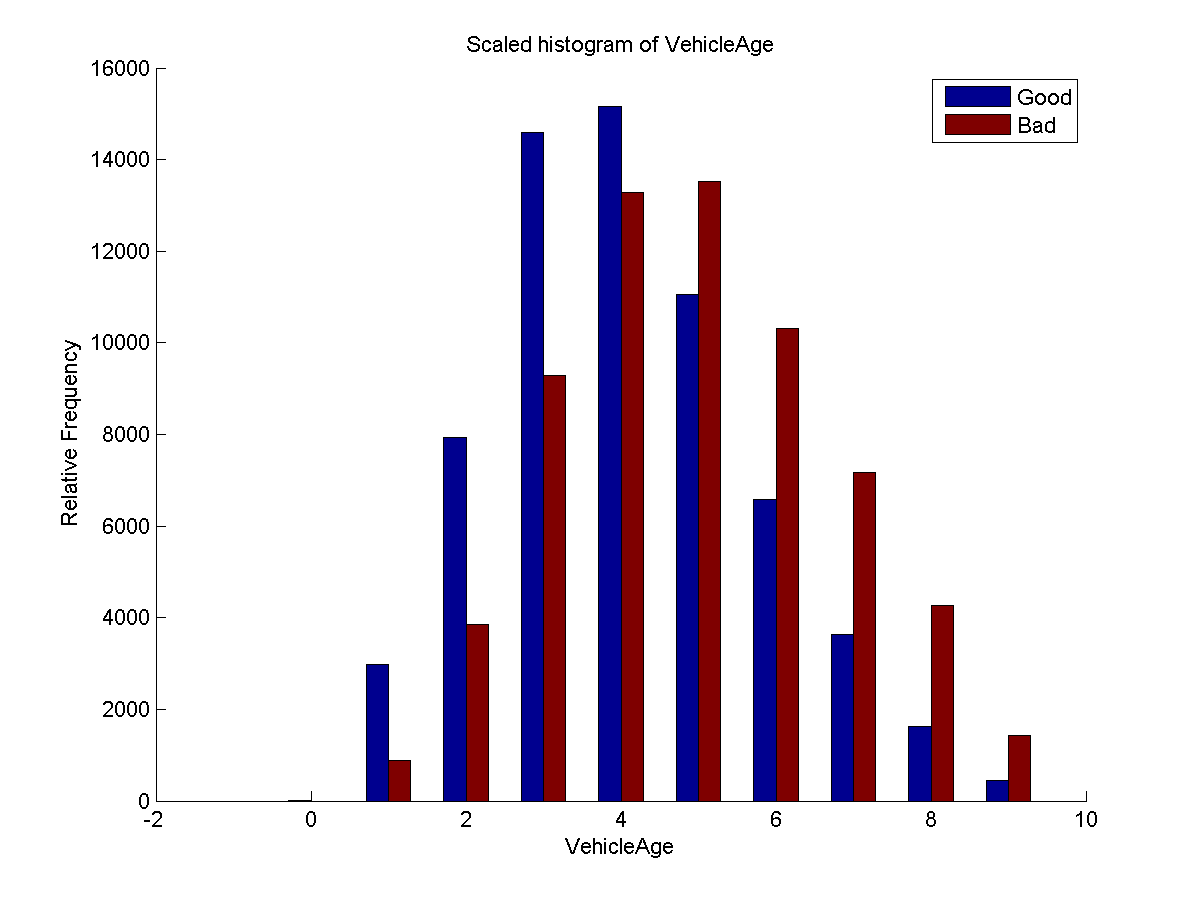
\includegraphics[width=\textwidth]{figures/HistogramScaled_VehicleAge.png}
                \caption{Ratio of Scaled VehicleAge}
                \label{fig:Scaled_VehicleAge}
        \end{subfigure}%
        ~ %add desired spacing between images, e. g. ~, \quad, \qquad etc. 
          %(or a blank line to force the subfigure onto a new line)
        \begin{subfigure}[b]{0.3\textwidth}
                \centering
                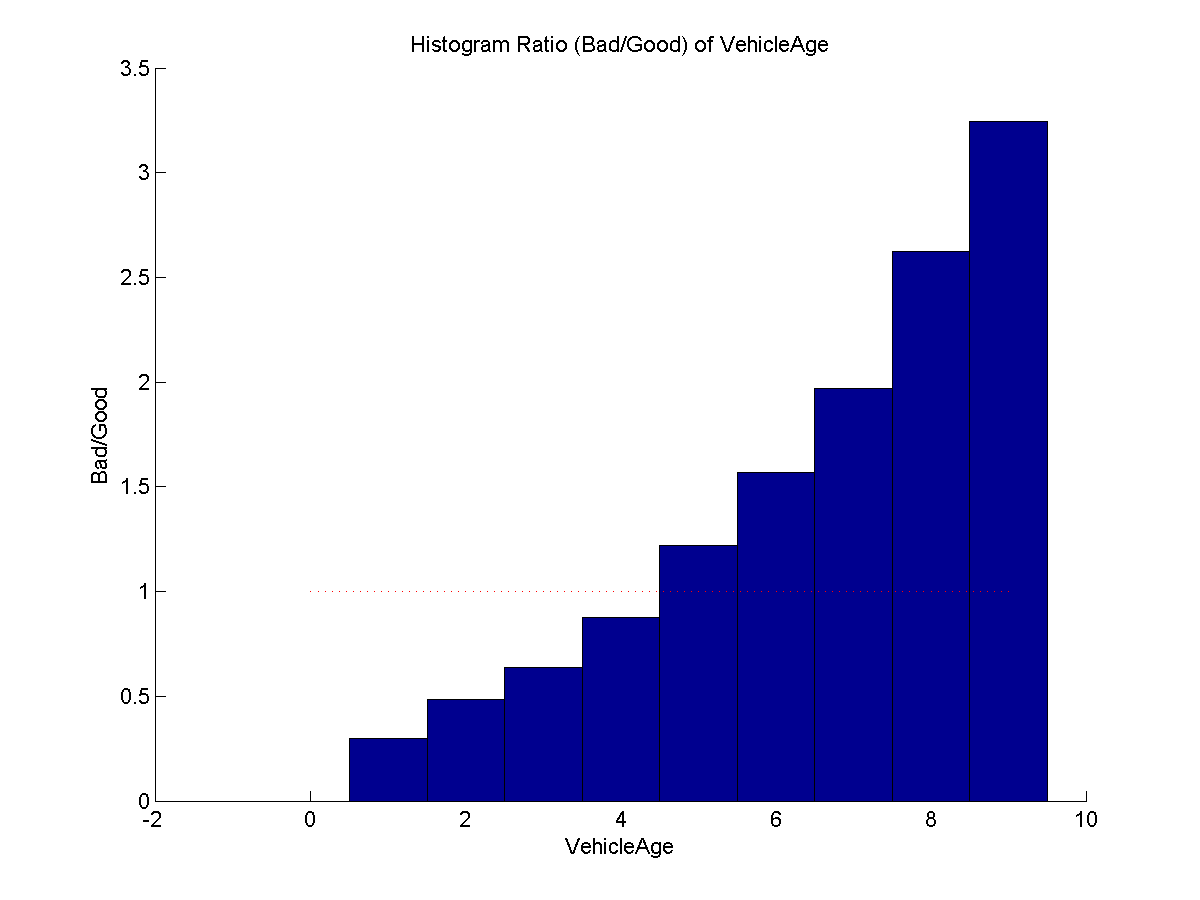
\includegraphics[width=\textwidth]{figures/HistogramRatio_VehicleAge.png}
                \caption{Ratio of VehicleAge}
                \label{fig:VehicleAge}
        \end{subfigure}
        ~ %add desired spacing between images, e. g. ~, \quad, \qquad etc. 
          %(or a blank line to force the subfigure onto a new line)
\begin{subfigure}[b]{0.3\textwidth}
					 \centering
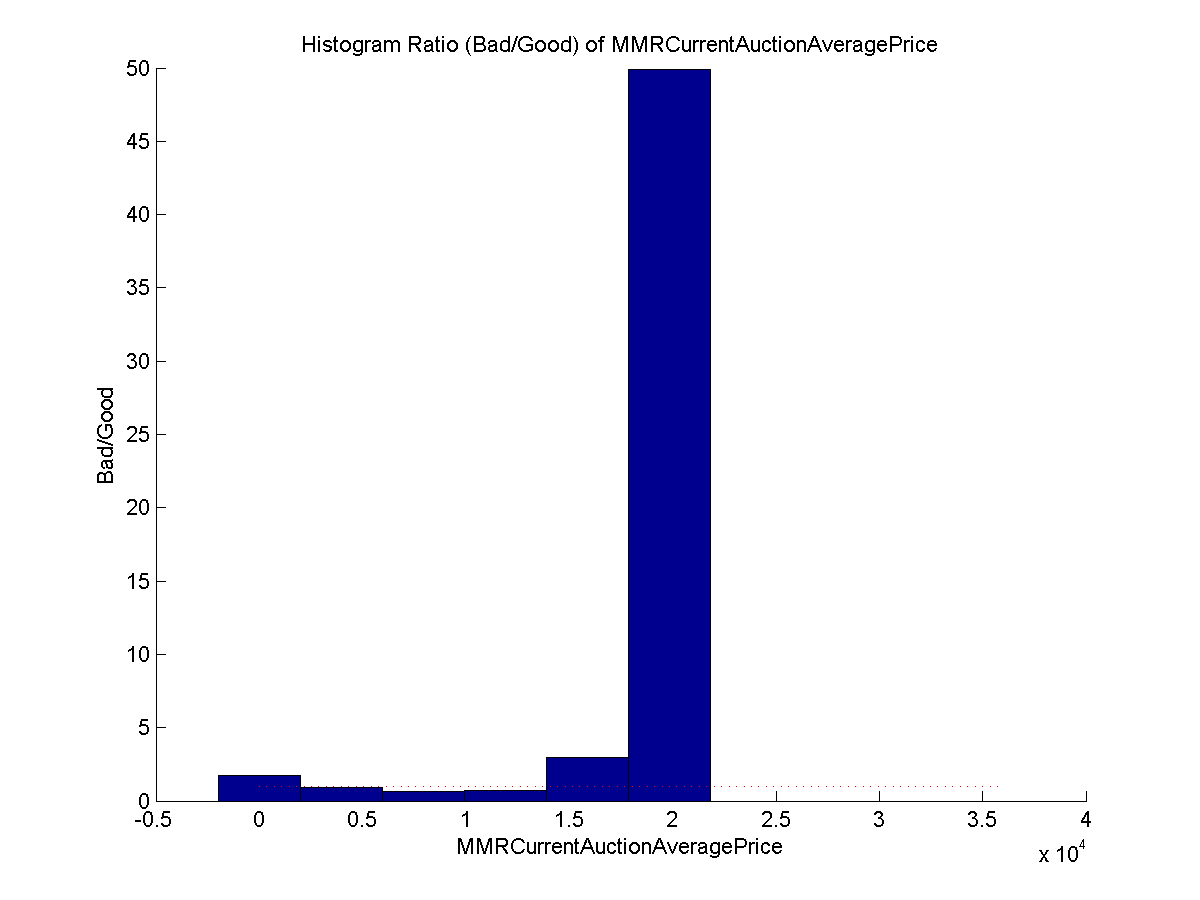
\includegraphics[width=\textwidth]{figures/HistogramRatio_MMRCurrentAuctionAveragePrice.png}
                \caption{Ratio of CurrAuctnAvgPrice}
                \label{fig:MMRCurrentAuctionAveragePrice}
        \end{subfigure}
        \caption{Histogram plots depicting ratio of scaled vehicle age, ratio of vehicle age, and current auction average price}\label{fig:Histograms}
\end{figure}
\end{comment}

\begin{thebibliography}{1}
\bibitem{Graf} Graf, A., & Borer, S. (2001). Normalization in support vector machines. Pattern Recognition, 277-282.

\bibitem{Menardi} Menardi G, Torelli N. (2010) {\em Training and assessing classi?cation rules with unbalanced data.} Working Paper Series

\bibitem{Provost} Provost, F. (2000) {\em Learning with Imbalanced Data Sets 101.} Invited paper for the AAAI'2000 Workshop on Imbalanced Data Sets.

\bibitem{Japkowicz} Japkowicz, N. (2000). {\em The Class Imbalance Problem: Signifcance and Strategies.} In Proceedings of the 2000 International Conference on Artifcial Intelligence (IC-AI�2000): Special Track on Inductive Learning Las Vegas, Nevada.

\bibitem{Friedman} Friedman, J., Hastie, T., & Tibshirani, R. (2000). {\em Additive logistic regression: a statistical view of boosting (With discussion and a rejoinder by the authors).} The annals of statistics, 28(2), 337-407.
 
\bibitem{Hastie} Hastie, T. (2003).  {\em Boosting.} Retrieved from Stanford University Web Site:  http://www.stanford.edu/~hastie/TALKS/boost.pdf
 
\bibitem{Dettling} Dettling, M., & B�hlmann, P. (2003). {\em Boosting for tumor classification with gene expression data.} Bioinformatics, 19(9), 1061-1069.
 
\bibitem{Caruana} Caruana, R., Niculescu-Mizil, A., Crew, G., & Ksikes, A. (2004, July). {\em Ensemble selection from libraries of models.} In Proceedings of the twenty-first international conference on Machine learning (p. 18). ACM.

\begin{comment}
\bibitem{notes} John W. Dower {\em Readings compiled for History
21.479.}  1991.

\bibitem{impj}  The 
Japan Reader {\em Imperial Japan 1800-1945} 1973:
Random House, N.Y.

\bibitem{norman} E. H. Norman {\em Japan's emergence as a modern
state} 1940: International Secretariat, Institute of Pacific
Relations.

\bibitem{fo} Bob Tadashi Wakabayashi {\em Anti-Foreignism and Western
Learning in Early-Modern Japan} 1986: Harvard University Press.
\end{comment}

\end{thebibliography}

\end{document}
